\documentclass[tikz,border=3mm]{standalone}

\usepackage{amsmath, amssymb, extarrows}


\usetikzlibrary{matrix,positioning,fit,backgrounds,intersections}
\usetikzlibrary{calc}
\usetikzlibrary{arrows}



\begin{document}

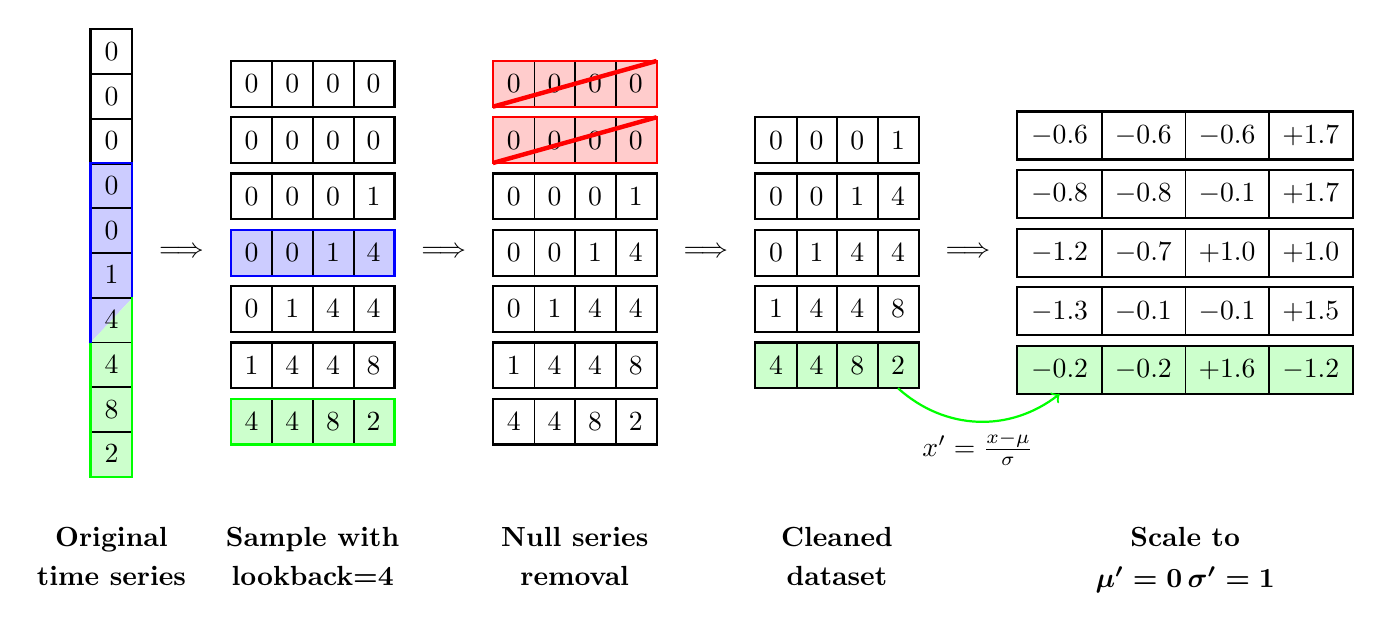
\begin{tikzpicture}[mmat/.style={matrix of math nodes,column sep=-\pgflinewidth/2,
   row sep=-\pgflinewidth/2,cells={nodes={draw,inner sep=5pt,ultra thin}},draw=#1,thick,inner sep=0pt},
   mmat/.default=black,
   node distance=0.3em]
 \matrix[mmat](ts_full){
         0 \\ 
         0 \\ 
         0 \\ 
         0 \\ 
         0 \\ 
         1 \\ 
         4 \\ 
         4 \\
         8 \\ 
         2 \\
         };
         
  \begin{scope}[on background layer]
  \fill[blue!20 ] (ts_full-4-1.north west) rectangle (ts_full-6-1.south east);
  \fill[green!20] (ts_full-8-1.north west) rectangle (ts_full-10-1.south east);
  \fill[blue!20]  (ts_full-6-1.south west) -- (ts_full-6-1.south east) --
                  (ts_full-7-1.south west) -- cycle;
  \fill[green!20] (ts_full-6-1.south east) -- (ts_full-7-1.south east) --
                  (ts_full-7-1.south west) -- cycle;
 \end{scope}       
 
    %bordo verde
   \draw[green, thick] (ts_full-7-1.south west) --
                       (ts_full-10-1.south west)--
                       (ts_full-10-1.south east)--
                       (ts_full-7-1.north east);
    %bordo blu
    \draw[blue, thick] (ts_full-7-1.south west) --
                       (ts_full-4-1.north west)--
                       (ts_full-4-1.north east)--
                       (ts_full-7-1.north east);
                  
\node[right=of ts_full] (lback) {$\implies$};

%central timeserie of preprocessed ones    
 \matrix[mmat, right=of lback , name path=ts_c0, fill=blue!20] (ts_c0) {0 & 0 & 1 & 4 \\ };
 %timeseries below central one
 \matrix[mmat, below=of ts_c0 , name path=ts_b1] (ts_b1) {0 & 1 & 4 & 4 \\ };
 \matrix[mmat, below=of ts_b1 , name path=ts_b2] (ts_b2) {1 & 4 & 4 & 8 \\ };
 \matrix[mmat, below=of ts_b2 , name path=ts_b3, fill=green!20] (ts_b3) {4 & 4 & 8 & 2 \\ };
 %timeseries above central one
 \matrix[mmat, above=of ts_c0 , name path=ts_a1] (ts_a1) {0 & 0 & 0 & 1 \\ };
 \matrix[mmat, above=of ts_a1 , name path=ts_a2] (ts_a2) {0 & 0 & 0 & 0 \\ };
 \matrix[mmat, above=of ts_a2 , name path=ts_a3] (ts_a3) {0 & 0 & 0 & 0 \\ };
 
 \node[fit=(ts_c0-1-1)(ts_c0-1-4),inner sep=0pt,draw,blue ,thick,name path=fit](f21){};
 \node[fit=(ts_b3-1-1)(ts_b3-1-4),inner sep=0pt,draw,green,thick,name path=fit](f22){};

 
 \node[right=of ts_c0] (nulls) {$\implies$};

%central timeserie of null removal     
 \matrix[mmat, right=of nulls , name path=ts_c0r] (ts_c0r)  {0 & 0 & 1 & 4  \\ };
 %timeseries below central one
 \matrix[mmat, below=of ts_c0r , name path=ts_b1r] (ts_b1r) {0 & 1 & 4 & 4  \\ };
 \matrix[mmat, below=of ts_b1r , name path=ts_b2r] (ts_b2r) {1 & 4 & 4 & 8  \\ };
 \matrix[mmat, below=of ts_b2r , name path=ts_b3r] (ts_b3r) {4 & 4 & 8 & 2  \\ };
 %timeseries above central one
 \matrix[mmat, above=of ts_c0r , name path=ts_a1r] (ts_a1r) {0 & 0 & 0 & 1  \\ };
 \matrix[mmat, above=of ts_a1r , fill=red!20, name path=ts_a2r] (ts_a2r) {0 & 0 & 0 & 0 \\ };
 \matrix[mmat, above=of ts_a2r , fill=red!20, name path=ts_a3r] (ts_a3r) {0 & 0 & 0 & 0 \\ };

 \node[fit=(ts_a3r-1-1)(ts_a3r-1-4),inner sep=0pt,draw,red,thick,name path=fit](f31){};
 \node[fit=(ts_a2r-1-1)(ts_a2r-1-4),inner sep=0pt,draw,red,thick,name path=fit](f32){};
 %sbarra le series nulle
 \draw[red, ultra thick] (ts_a3r-1-1.south west) --(ts_a3r-1-4.north east);
 \draw[red, ultra thick] (ts_a2r-1-1.south west) --(ts_a2r-1-4.north east);


 \node[right=of ts_c0r] (nulls2) {$\implies$};

%central timeserie of cleaned ones     
 \matrix[mmat, right=of nulls2 , name path=ts_c0c] (ts_c0c) {0 & 1 & 4 & 4  \\ };
 %timeseries below central one
 \matrix[mmat, below=of ts_c0c , name path=ts_b1c] (ts_b1c) {1 & 4 & 4 & 8  \\ };
 \matrix[mmat, below=of ts_b1c , fill=green!20, name path=ts_b2c] (ts_b2c) {4 & 4 & 8 & 2  \\ };
 %timeseries above central one
 \matrix[mmat, above=of ts_c0c , name path=ts_a1c] (ts_a1c) {0 & 0 & 1 & 4  \\ };
 \matrix[mmat, above=of ts_a1c , name path=ts_a2c] (ts_a2c) {0 & 0 & 0 & 1   \\ };

 \node[right=of ts_c0c] (scale) {$\implies$};

%central timeserie of scaled ones     
 \matrix[mmat, right=of scale  , name path=ts_c0r] (ts_c0s) {-1.2 & -0.7 & +1.0 & +1.0 \\ };
 %timeseries below central one
 \matrix[mmat, below=of ts_c0s , name path=ts_b1s] (ts_b1s) {-1.3 & -0.1 & -0.1 & +1.5 \\};
 \matrix[mmat, below=of ts_b1s , fill=green!20, name path=ts_b2s] (ts_b2s) {-0.2 & -0.2 & +1.6 & -1.2 \\};
 %timeseries above central one
 \matrix[mmat, above=of ts_c0s , name path=ts_a1s] (ts_a1s) {-0.8 & -0.8 & -0.1 & +1.7 \\ };
 \matrix[mmat, above=of ts_a1s , name path=ts_a2s] (ts_a2s) {-0.6 & -0.6 & -0.6 & +1.7 \\ };
 

 
 
 
  \path (ts_full.south)   node[below=0.5] {\textbf{Original}}
  (ts_c0|-ts_full.south)  node[below=0.5] {\textbf{Sample with}}
  (ts_c0r|-ts_full.south) node[below=0.5] {\textbf{Null series}}
  (ts_c0c|-ts_full.south) node[below=0.5] {\textbf{Cleaned}}
  (ts_c0s|-ts_full.south) node[below=0.5] {\textbf{Scale to}};
  
  \path (ts_full.south)   node[below=1.0] {\textbf{time series}}
  (ts_c0|-ts_full.south)  node[below=1.0] {\textbf{lookback=4}}
  (ts_c0r|-ts_full.south) node[below=1.0] {\textbf{removal}}
  (ts_c0c|-ts_full.south) node[below=1.0] {\textbf{dataset}}
  (ts_c0s|-ts_full.south) node[below=1.0] {\textbf{$\boldsymbol{\mu^\prime=0\,\sigma^\prime=1}$}};


    \draw[->, green, thick] (ts_b2c-1-4.south) to [bend right=40]
     node[below] {\textcolor{black}{$x^\prime=\frac{x-\mu}{\sigma}$}}(ts_b2s-1-1.south);
  
 
  
\end{tikzpicture}

\end{document}